\documentclass[]{beamer}
\usetheme{default}

\usepackage{graphicx} % \includegraphics
\usepackage{mathrsfs} % \mathscr

% to print with notes
%\setbeameroption{show notes}

% no decoration to notes
%\setbeamertemplate{note page}[plain]

% http://tex.stackexchange.com/questions/66995/modify-footer-of-slides
\makeatother
\setbeamertemplate{footline}
{
  \leavevmode
  \hbox{
  \begin{beamercolorbox}[wd=.4\paperwidth,ht=2.25ex,dp=1ex,center]{author in head/foot}
    \usebeamerfont{author in head/foot}\insertshortauthor
  \end{beamercolorbox}
  \begin{beamercolorbox}[wd=.6\paperwidth,ht=2.25ex,dp=1ex,center]{title in head/foot}
    \usebeamerfont{title in head/foot}\insertshorttitle\hspace*{3em}
    \insertframenumber{} / \inserttotalframenumber\hspace*{1ex}
  \end{beamercolorbox}}
  \vskip0pt
}
\makeatletter
\setbeamertemplate{navigation symbols}{}

\begin{document}

\title{Cluster algorithms for the Ising model}
\author{Roger Walt}

\begin{frame}
	\huge{Cluster algorithms for the Ising model}
	\vspace*{5pt}

	\Large{Monte Carlo methods which overcome the problem of critical slowing down close to second order phase transitions}
\end{frame}

\begin{frame}{Contents}
\begin{itemize}
\item Ising model
\item Single spin flip metropolis
\item Autocorrelation, Binning Analysis
\item Wolff algorithm
\item Swensen-Wang algorithm
\end{itemize}
\end{frame}

\begin{frame}{Ising model}
\begin{columns}[c]
	\column{.5\textwidth}
	\begin{itemize}
		\item<2-> Phase transitions
			\note[item]<1> {Phase transitions are important}
		\item<3-> One of the simplest statistical models that show a phase transition
			\note[item]<2> {The Ising model is one of the simplest statistical models that shows a phase transition.}
		\item<4-> Magnetic systems, opinion models, binary mixtures
			\note[item]<3> {Ising model can be used to simulate magnetic systems (ferromagnetic and antiferromagnetic), opinion models and binary mixtures.}
	\end{itemize}
	\column{.5\textwidth}
	\pause[5]
	\begin{figure}[p]
		\centering
		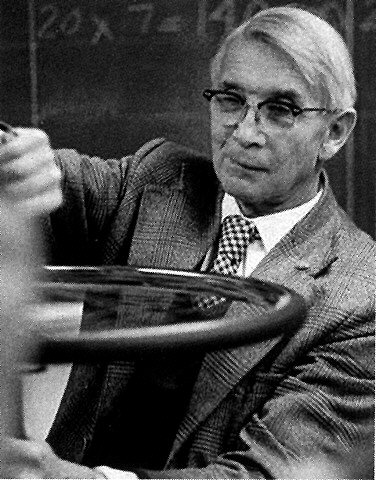
\includegraphics{img/ising.jpg}
		\caption{Ernst Ising (1900 - 1998)}
		\label{fig:awesome_image}
	\end{figure}
	\note<4> {Figure: Ernst Ising, lived from 1900 to 1998}
	\note[item]<4> {Ising model invented by Wilhelm Lenz (1888 - 1957) (the same as the Lenz in the Laplace-Runge-Lenz vector) in 1920, his student Ernst Ising solved it in the one-dimensional case 1924.}
	\note[item]<4> {Wolfgang Pauli (1900 - 1958), at whom the road outside is named after, was an assistant of Lenz.}
	\note[item]<4> {Also Otto Stern (1888 - 1969) from the Stern-Gerlach experiment was an assistant of Lenz.}
\end{columns}
\end{frame}

\begin{frame}{Ising model - Definition}
\begin{itemize}
	\note[item]<1> {Lattice with \(N\) sites.}
\item<2-> Discrete integer spins \( \sigma_i = \pm 1 \) on each lattice site
\end{itemize}
\pause[3]
\[ \mathscr{H}(\sigma) = -J \sum\limits_{\left< i, j \right>} \sigma_i \sigma_j - H \sum\limits_i \sigma_i \]
	\note[item]<4> {Sum over nearest neighbours.}
	\note[item]<4> {\( J \): interaction, \( H \): external field}
	\note[item]<4> {\( J_{ij} \) in general case, \( J>0 \): ferromagnetic, \( J<0 \): antiferromagnetic}

\begin{columns}[c]
	\column{.5\textwidth}
	\pause
	\def\svgwidth{.5\textwidth}
	\centering
	\input{img/spins_parallel.pdf_tex}
	\column{.5\textwidth}
	\pause
	\def\svgwidth{.5\textwidth}
	\centering
	\input{img/spins_antiparallel.pdf_tex}
		\note[item]<5> {For positive J: More favorable for the spins to be aligned!}
\end{columns}
\end{frame}

\begin{frame}{Ising model - Canonical ensemble}
\pause
\[ p(\sigma, T) = \frac{e^{-\beta \mathscr{H}(\sigma)}}{\mathscr{Z}(T)}, \ \ \ \ \beta=\frac{1}{k_B T}\]
	\note[item]<2> {Configuration probability given by boltzmann distribution, Z partition function, given as \[ \mathscr{Z}(T) = \sum_\sigma e^{-\beta \mathscr{H}(\sigma)},\ \ \beta = \frac{1}{k_B T} \]}
	\note[item]<2> {So we are looking at a canonical system with constant temperature T.}
\pause
\[ \left< M \right>_T = \sum_\sigma M(\sigma)p(\sigma,T) \]
	\note[item]<3> {Measurement value of a function, e.g. magnetization, is given by the sum over all states of the measurement value at the configuration times the configuration probability.}
\end{frame}

\begin{frame}{Ising model - Monte Carlo}
\begin{itemize}
\item<2-> We can't compute all configurations (\(2^N\))
	\note[item]<2> {Why not? \( \rightarrow 2^N = 2^{L^d} \) e.g. \( L = systemSize = 15 \) in 2 dimensions: \(2^{15^2} = 2^{225} = 5 \cdot 10^{67}\)}
	\note[item]<2> {We can't compute the exact expectation value of an observable. But that's what we're interested in.}
\item<3-> We can't sample uniformely distributed over energy \def\svgwidth{12em} \input{img/energy_gaussian.pdf_tex}
	\note[item]<3> {Because the distribution of the average energy gets sharper with increasing size \(\left(\alpha \ \sqrt{L^d}\right)\).}
\item<4-> Solution: Importance sampling using Metropolis algorithm
\end{itemize}
\end{frame}

\begin{frame}{Single spin flip metropolis - Algorithm}

\begin{align*}
\visible<4->{A(X \rightarrow Y) &= \min \left( 1, \frac{p(Y)}{p(X)} \right) \\}
\visible<5-> {
&= \min \left( 1, e^{- \beta \left[ E(Y)-E(X) \right] } \right)}
\end{align*}

\note {If energy decreases, always accept. If energy increases, accept with probability \( e^{- \beta \Delta E} \).}
\begin{enumerate}
\item<2-> Choose one site (uniformly randomly)
	\note[item] {New state given by spinflip at this site.}
\item<3-> Generate new trial configuration Y by flipping spin
\item<4-> Accept new configuration with transition probability above
\end{enumerate}
\note{Blazingly fast (Troells: 2 flips/ns?), easy to implement.}
\end{frame}

\begin{frame}{Single spin flip metropolis - Results}
\pause
Magnetization \( M(T) = \left< \frac{1}{N} \sum\limits_{i=1}^N \sigma_i \right>_T \)
\begin{columns}[c]
	\column{.5\textwidth}
	\pause
	\centering Expected
	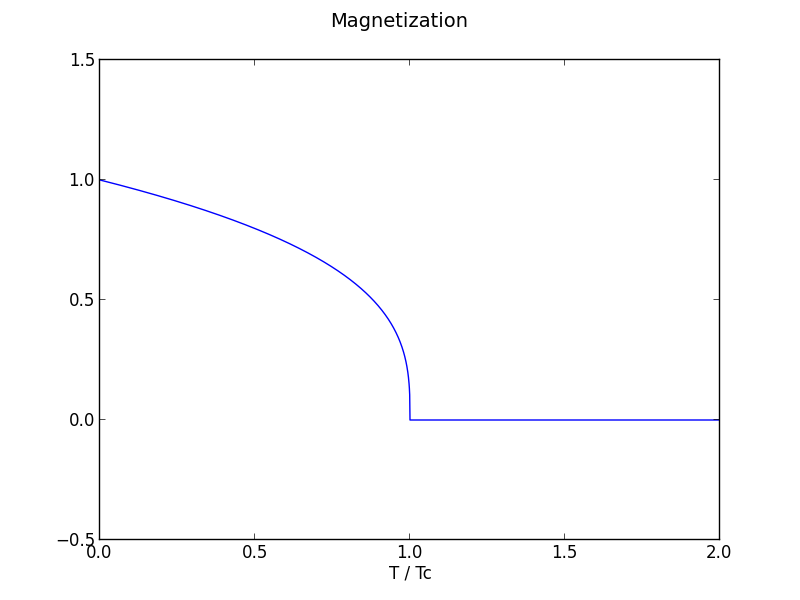
\includegraphics[width=\textwidth]{img/single_magnetization_theoretical.png}
	\column{.5\textwidth}
	\pause
	\centering Obtained
	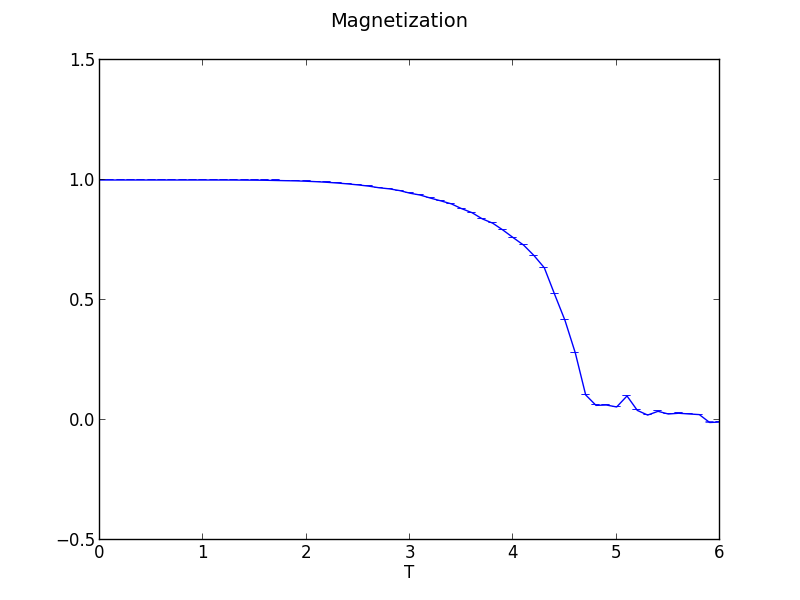
\includegraphics[width=\textwidth]{img/single_magnetization_size15.png}
\end{columns}
\note[item]<1> {I implemented this single spin flip metropolis algorithm and would like to show you some results.}
\note[item]<2> {Let's look at the spontaneous magnetization.}
\note[item]<3> {In theory, we expect a spontaneous magnetization below \(T_C\). We expect a symmetry breaking (either positive or negative Magnetization in this case) and a discontinuity in the derivative of the magnetization at \(T_C\). We want something linear to \( (T-T_C)^\nu \).}
\note[item]<4> {Well, this is what we get. It looks perfect - right? We see a spontaneous magnetization in the simulation. The discontinuity in its derivative is not there, but this is okay, since we are looking at a finite sized system.
Well, life is not so easy. This result is in fact not the truth. Let me show you what we expect for the spontaneous magnetization.}
\end{frame}

\begin{frame}{Ising model - 2 spins}
\note{Show that we should expect the magnetization to vanish.}
\end{frame}

\begin{frame}{Single spin flip metropolis - To flip or not to flip}
\pause
\[ \mathscr{H}(\sigma) = -J \sum\limits_{\left< i, j \right>} \sigma_i \sigma_j \]
\note[item]<1> {Now that we know that the magnetization should vanish, let's explore why it hasn't done so.}
\note[item]<2> {The hamiltonian of the system states clearly that the spins like to be aligned. They were all +1 at the beginning, and then thermalized (brought to thermodynamic equilibrium) in 3 sweeps (abbrevation for: 3 times number of sites spinflips).}
\note[item]<2> {The point is that the spins can also be aligned when they are all -1. But we didn't see that happen. Why?}
\note[item]<2> {I took 0.5 million measurement values, after every single spin flip. This means that the spin on every site could have flipped around 150 times. But it didn't. This is why:}
\pause
\centering
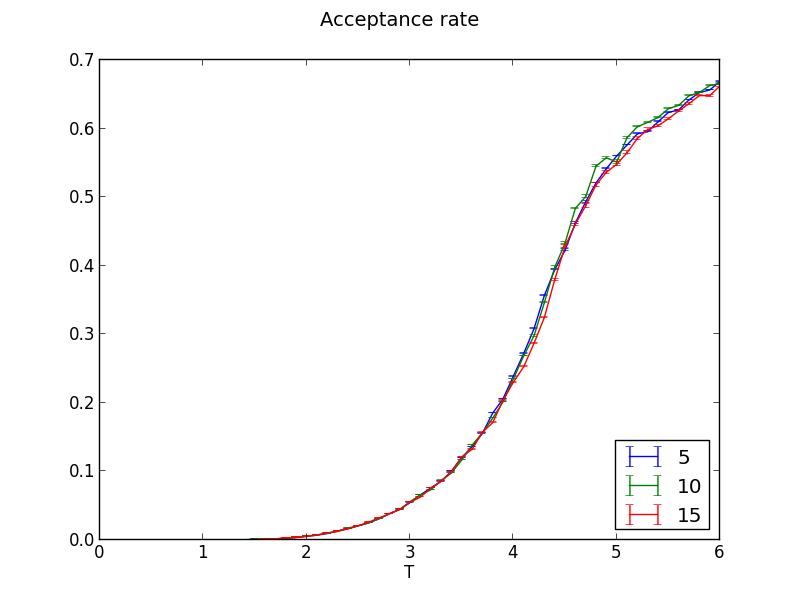
\includegraphics[height=12em]{img/single_acceptanceRate.png}
	\note[item]<3> {What we see here is the acceptance rate of a spin flip. It is one if the suggested new configuration through the single spin flip was accepted. Well, it's actually almost zero for low temperatures. So we move ultra slow through phase space, which is no fun, because we want to do an ergodic sampling.}
\note[item]<3> {\[ \frac{N}{a(T)} = \text{\# trials} \]}
\note[item]<3> {We want to change flip the magnetization of the system completely at least 100 times to have good statistics. For uncorrelated measurements we then have an error of 10\%.}
\end{frame}

\begin{frame}{Autocorrelation time}
\note[item]<1> {There is another approach to describe what's going on. Not accepting a spinflip or only flipping one spin at a time means that the new configuration is highly correlated to the old one.}
\pause
\[ \phi_{A}(t) = \frac{\left< A(t_0)A(t) \right> - \left< A \right>^2}{\left< A(t_0)^2 \right> - \left< A \right>^2} \visible<3->{\propto e^{-\frac{t}{\tau_A}}} \]
\note[item]<2> {We define the linear autocorrelation function of a measurement value as a ratio of the covariance of two observables at a given point in time and at time \(t_0\).}
\begin{columns}[c]
	\column{.5\textwidth}
	\pause[4]
	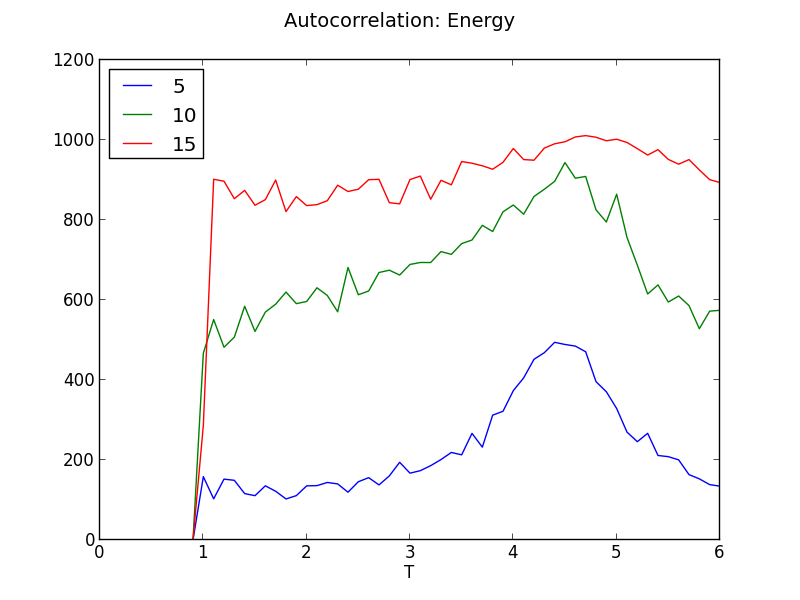
\includegraphics[width=\textwidth]{../results/measurements/autocorr_energy_single.png}
	\column{.5\textwidth}
	\pause[5]
	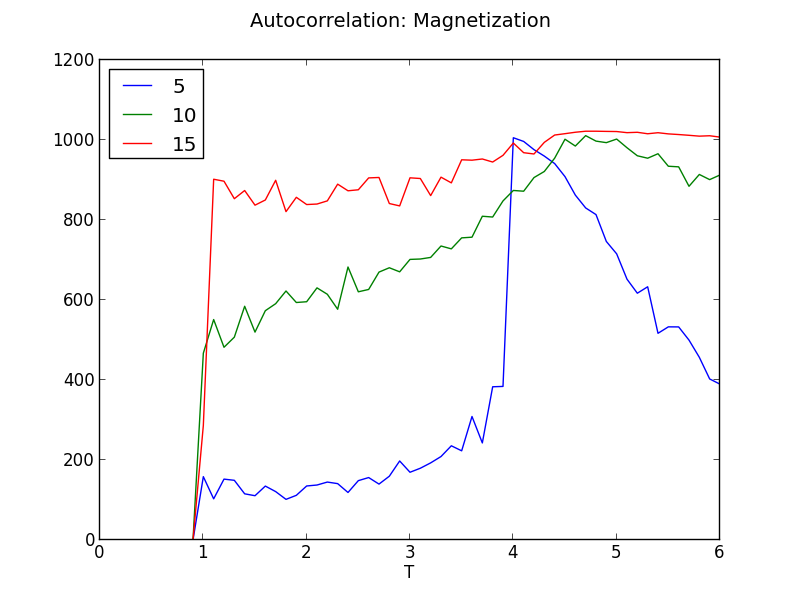
\includegraphics[width=\textwidth]{../results/measurements/autocorr_magnetization_single.png}
\end{columns}
\note[item]<3> {We see that the energy converges much faster than the magnetization. I read that people often focus on the energy, but here you really have to focues on the magnetization to be sure.}
\note{Definition and plots from measurements, magnetization and energy.}
\end{frame}

\begin{frame}{Binning analysis I}
\pause
\[ \text{Var} X := E \left[ X^2 \right] - E \left[ X \right]^2 \]
\pause
\[ (\Delta X)^2 = \frac{\text{Var}X}{N}\left(1+2\tau_X\right) \]
\note{For uncorrelated samples we know: \[ E\left[X_i X_j \right] = E\left[X_i\right] E\left[X_j\right] \text{ for } i \neq j \]
The correlation time of a variable is defined as:
\[ \tau_X := \frac{\sum\limits_t \left( E\left[ X_i X_{i+t} \right]-E \left [X \right] ^2 \right)}{\text{Var}X} \]}
\end{frame}

\begin{frame}{Binning analysis II}
\pause
\[ A_i^{(l)} = \frac{1}{2} \left( A_{2i-1}^{(l-1)} + A_{2i}^{(l-1)} \right) \]
\pause
\[ \Delta^{(l)} = \sqrt{\text{Var}A^{(l)}/M^{(l)}}  \stackrel{l \rightarrow \infty}{\rightarrow} \Delta = \sqrt{(1+2\tau_A)\text{Var}A/M} \]
\pause
\[ \tau_A = \lim_{l\rightarrow\infty}\left( \frac{2^l \text{Var} A^{(l)}}{\text{Var} A^{(0)}} - 1 \right) \]
\note{Draw graphics with the bins and the levels.}
\end{frame}

\begin{frame}{What really happens in the System}
\note{Draw domains on board and show single spin flip only is useful at borders of domains.}
\end{frame}

\begin{frame}{Cluster algorithms: Wolff algorithm}
\[ P(\sigma_x, \sigma_y) = 1 - \min \left( 1,e^{2\beta \sigma_x \sigma_y} \right) \]
\begin{enumerate}
\item<2-> Choose one site (uniformly randomly)
\item<3-> Flip its spin and add it to the cluster
\item<4-> For all sites in the cluster:
	\begin{enumerate}
	\item Visit every unknown neighbour, flip its spin and add it to the cluster with probability given above
	\end{enumerate}
\end{enumerate}
\end{frame}

\begin{frame}{Why cluster algorithms are better}
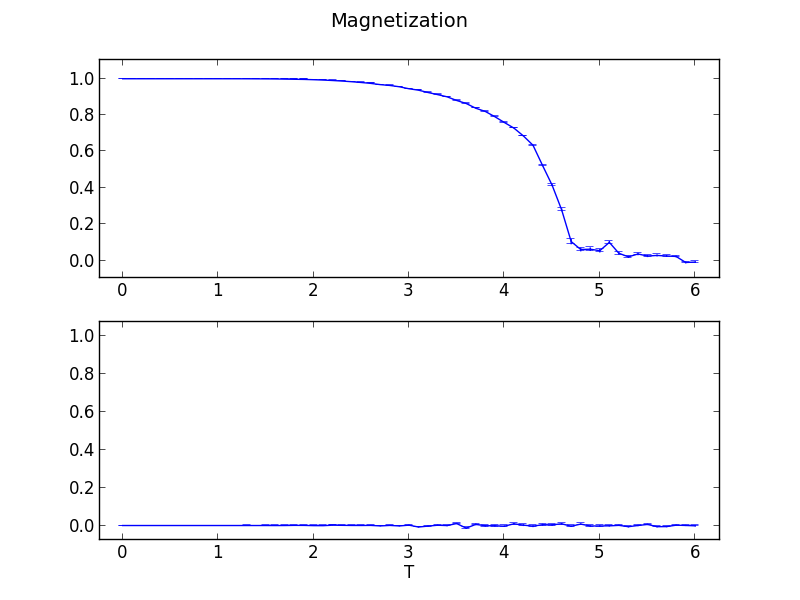
\includegraphics[width=\textwidth]{img/comp_magnetization.png}
\end{frame}

\begin{frame}{Energy}
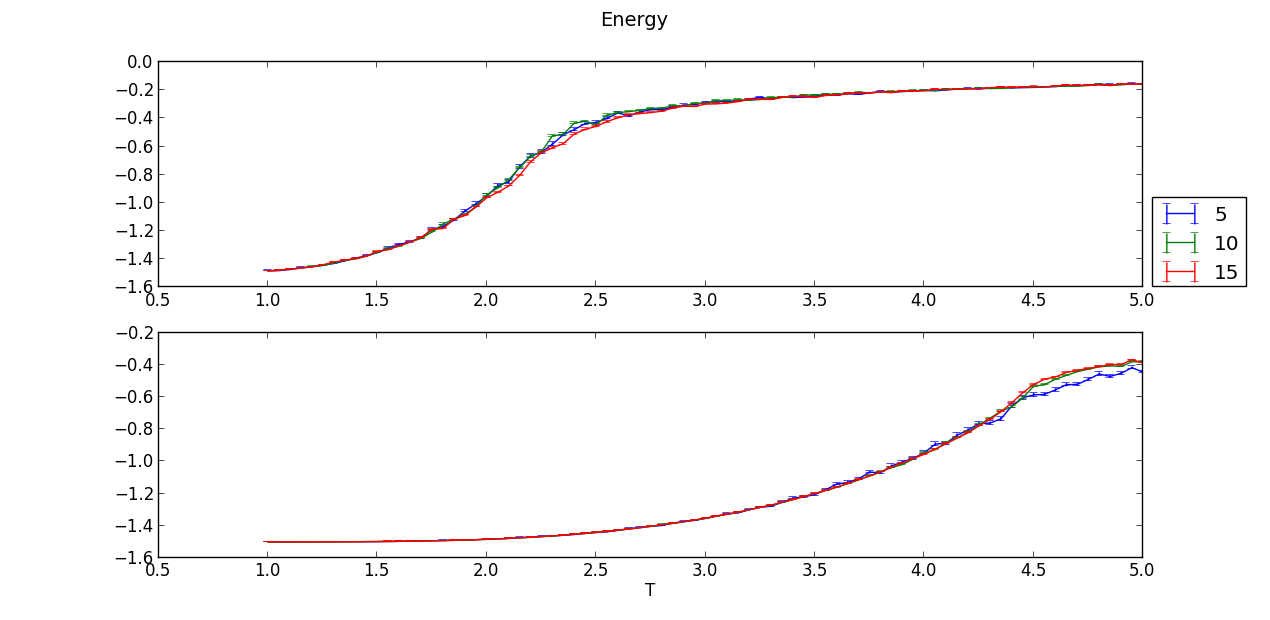
\includegraphics[width=\textwidth]{../results/measurements/energy.png}
\end{frame}

\begin{frame}{Cluster size}
\end{frame}

\begin{frame}{Magnetization}
\end{frame}

\begin{frame}{Magnetization squared}
\note{Magnetization itself is a bad order parameter, since it can have two signs so it cancels. Magnetization squared is a good order parameter, because it consists of sums of spatial spin correlations. It shows the phase transition.}
\end{frame}

\begin{frame}{Computation time per spin flip}
\end{frame}

\begin{frame}{Swendsen-Wang}
\end{frame}


\begin{frame}
\centerline{\huge{Questions}}
\end{frame}

\begin{frame}{Binning analysis in detail}
\[ \text{Var} X := E \left[ X^2 \right] - E \left[ X \right]^2 \]
\begin{align*}
(\Delta X)^2 &= \frac{1}{N^2} \sum\limits_{i,j=1}^N \left( E \left[ X_i X_j \right] - E \left[ X \right]^2 \right) \\
&= \frac{\text{Var}X}{N}+\frac{1}{N^2}\sum\limits_{i\neq j} \left( E \left[X_i X_j \right] - E \left[ X \right]^2 \right) \\
&= \frac{\text{Var}X}{N}+\frac{2}{N^2}\sum\limits_{i=1}^N \sum\limits_t \left( E\left[X_i X_{i+t} \right] - E \left[ X \right]^2 \right) \\
&:= \frac{\text{Var}X}{N}\left(1+2\tau_X\right)
\end{align*}
\note{For uncorrelated samples we know: \[ E\left[X_i X_j \right] = E\left[X_i\right] E\left[X_j\right] \text{ for } i \neq j \]
The correlation time of a variable is defined as:
\[ \tau_X := \frac{\sum\limits_t \left( E\left[ X_i X_{i+t} \right]-E \left [X \right] ^2 \right)}{\text{Var}X} \]}
\end{frame}

\begin{frame}{Wolff or Swendsen-Wang?}
Swendsen-Wang better for parallelization because it touches the whole lattice.
\end{frame}

\end{document}
